\documentclass[11pt]{article}

\usepackage[utf8]{inputenc}
\usepackage[T1]{fontenc}
\usepackage{amsmath,amssymb}
\usepackage{graphicx}
\usepackage{booktabs}
\usepackage{natbib}
\usepackage[breaklinks=true]{hyperref}
\usepackage{url}
\Urlmuskip=0mu plus 1mu
\usepackage{xcolor}
\usepackage{geometry}
\usepackage{float}
\usepackage{multirow}
\usepackage{caption}
\usepackage{subcaption}
\usepackage{algorithm}
\usepackage{algpseudocode}
\usepackage{setspace}

\geometry{margin=1in, headheight=15pt}
\bibliographystyle{abbrvnat}
\setcitestyle{authoryear,open={(},close={)}}

% Better spacing
\setstretch{1.0}
\raggedbottom

% Section spacing
\usepackage{titlesec}
\titlespacing*{\section}{0pt}{1.2\baselineskip}{0.8\baselineskip}
\titlespacing*{\subsection}{0pt}{1.0\baselineskip}{0.6\baselineskip}
\titlespacing*{\subsubsection}{0pt}{0.9\baselineskip}{0.5\baselineskip}

% Caption styling
\captionsetup{font=small,labelfont=bf,margin=10pt}
\captionsetup[sub]{font=small}

% Figure spacing
\setlength{\floatsep}{12pt}
\setlength{\textfloatsep}{12pt}
\setlength{\intextsep}{12pt}

\title{A Pioneering AI Land Surface Model for Subseasonal-to-Seasonal Prediction}

\author{\parbox{0.9\textwidth}{%
\centering
Manmeet Singh$^{1}$, Nachiketa Acharya$^{2}$, Priyanka Yadav$^{3,4}$, Josh Durkee$^{1}$, \\
Somnath Luitel$^{1}$, Sanjiv Kumar$^{5}$, Zong-Liang Yang$^{7}$, Cenlin He$^{6}$, \\
Naveen Sudharsan$^{7}$, Harsh Kamath$^{8}$, Mahmoud Mbarak$^{9}$, \\
Prabhjot Singh$^{7}$, Amit Srivastava$^{10}$
\\[12pt]
{\small
$^{1}$Department of Earth, Environmental and Atmospheric Sciences, Western Kentucky University, Bowling Green, KY \\
$^{2}$Spire Global, Inc. \\
$^{3}$Earth System Science Interdisciplinary Center (ESSIC), University of Maryland, College Park, MD \\
$^{4}$NASA Goddard Space Flight Center, Greenbelt, MD \\
$^{5}$Auburn University, Auburn, AL \\
$^{6}$National Center for Atmospheric Research (NCAR), Boulder, CO \\
$^{7}$The University of Texas at Austin, Austin, TX \\
$^{8}$National Oceanic and Atmospheric Administration (NOAA) \\
$^{9}$Duke University, Durham, NC \\
$^{10}$Leibniz Centre for Agricultural Landscape Research (ZALF), Berlin, Germany \\[8pt]
Corresponding author: \texttt{manmeet.singh@wku.edu}
}
}}

\date{\today}

\begin{document}
\maketitle

% =====================================================================
\begin{abstract}
Land surface processes govern critical memory mechanisms---soil moisture, soil temperature, and snow---that underpin subseasonal-to-seasonal (S2S) predictability. However, the recent revolution in AI-based weather and climate models has focused almost exclusively on the atmosphere, leaving no modular AI land surface model available for coupling with other AI components. We present the first standalone AI land surface model designed as a modular component for coupled AI earth system modeling. The model is trained on ERA5 reanalysis data (native resolution 0.25$^\circ$), regridded to a global Hierarchical Equal Area isoLatitude Pixelisation (HEALPix) grid at 0.7$^\circ$ resolution for processing, taking 9 atmospheric forcing variables and 8 soil state variables at time $t$ and predicting the land surface state at time $t+1$ (one day ahead): soil moisture across 4 soil layers and soil temperature across 4 levels. Data are accessed via cloud-native infrastructure, requiring no local downloads. In offline prediction mode---where observed atmospheric forcing from ERA5 is provided at each time step while the model evolves its own land surface state---the model produces skillful 60-day forecasts of soil moisture and soil temperature, validated across four extreme events: the 2019 Mississippi River basin flooding, the 2012 Central US drought, the 2021 Pacific Northwest heat dome, and the 2011 Texas drought, spanning 16 initializations. The model maintains anomaly correlation coefficients above 0.5 beyond 30 days for surface soil moisture, demonstrating its viability as the land component of coupled AI S2S prediction systems and offering the potential to be integrated into any physics-based or AI-based coupled model.
\end{abstract}

% =====================================================================
\section{Introduction}
\label{sec:intro}

The land surface exerts a profound influence on weather and climate across a wide range of timescales. Soil moisture, in particular, acts as a source of predictability at subseasonal-to-seasonal (S2S) scales through its control on the partitioning of surface energy and water fluxes \citep{koster2004glace, seneviratne2010landclimate, dirmeyer2011landatm}. The Global Land--Atmosphere Coupling Experiment (GLACE) demonstrated that realistic soil moisture initialization can improve precipitation forecast skill weeks into the future \citep{koster2004glace}. Soil temperature, though less studied in this context, similarly provides memory through its coupling with surface energy balance and freeze--thaw processes. These land surface memory mechanisms are central to S2S prediction \citep{vitart2017s2s, merryfield2020s2s}.

Over the past four decades, the geoscience community has developed sophisticated physics-based land surface models (LSMs) to represent these processes. Models such as Noah-MP \citep{niu2011noahmp, ek2003noah}, the Community Land Model (CLM5; \citealt{lawrence2019clm5}), and the Joint UK Land Environment Simulator (JULES; \citealt{best2011jules}) solve coupled energy and water balance equations across multiple soil layers, incorporating vegetation dynamics, snow physics, and increasingly, groundwater and biogeochemical cycles. These models are typically developed and validated in offline mode---driven by observed or reanalysis atmospheric forcing---before being coupled into general circulation models (GCMs) for weather and climate prediction \citep{bauer2015quietrev}.

Concurrently, the past five years have witnessed a revolution in AI-based weather prediction. Beginning with early demonstrations using convolutional neural networks \citep{weyn2019dlwp, weyn2020dlwpcs}, the field rapidly advanced through Pangu-Weather \citep{bi2023pangu}, GraphCast \citep{lam2023graphcast}, FourCastNet \citep{pathak2022fourcastnet}, Spherical Fourier Neural Operators \citep{bonev2023sfno}, FuXi \citep{chen2023fuxi}, and Aurora \citep{bodnar2024aurora}. These models have demonstrated forecast skill competitive with---and in many metrics exceeding---operational numerical weather prediction systems such as ECMWF's Integrated Forecasting System, as documented by the WeatherBench~2 benchmark \citep{rasp2024weatherbench2}. More recently, NeuralGCM has shown that AI-based atmospheric dynamics can be combined with physical parameterizations for stable long-term climate simulations \citep{kochkov2024neuralGCM}.

A critical observation, however, is that nearly all of these AI weather models operate exclusively on atmospheric variables. They do not contain separate, identifiable land surface components. While some models (e.g., NeuralGCM) include land surface embeddings within their architectures, these are not modular components that can be independently developed, validated, or coupled. The first coupled AI ocean--atmosphere model, OLA \citep{caillon2024ola}, demonstrated the viability of training separate AI models for ocean and atmosphere on a shared grid and coupling them at inference time---but did not include a land component. Similarly, efforts in AI-based S2S prediction, such as FuXi-S2S \citep{chen2024fuxis2s}, have begun incorporating land surface variables but without a standalone, separable land model component.

This gap motivates the present work. We introduce the first standalone AI land surface model designed as a modular component for coupled AI earth system modeling. No such AI-based land surface model existed prior to this work. The model is explicitly designed to be modular: it can be integrated into any coupled AI or physics-based forecasting system that operates on a compatible grid. Following the time-honored development philosophy of physics-based LSMs---offline validation before coupled integration---we present the model in offline mode, forced by ERA5 atmospheric reanalysis data. The model is built as part of the Earthmind S2S framework, which aims to couple independent AI models for atmosphere, land, and ocean on a common grid.

The key contributions of this work are:
\begin{enumerate}
    \item The first standalone AI land surface model, which did not exist in the literature prior to this work. The model fills a critical gap in coupled AI earth system modeling.
    \item A neural network architecture adapted for global land surface modeling on a global equal-area grid, treating the 12 grid faces as a depth dimension in 3D convolutions, enabling shared-grid coupling with AI atmosphere and ocean models.
    \item A cloud-native training pipeline that streams ERA5 reanalysis data directly from cloud-optimized storage, eliminating the need for local data infrastructure.
    \item Demonstration of skillful autoregressive offline forecasts of soil moisture and soil temperature out to 60 days across four high-impact extreme events (flooding, drought, heat) at S2S timescales.
    \item An open, modular design that enables the model to be plugged directly into any coupled forecasting system---whether physics-based or AI-based---with minimal adaptation, advancing the modularity paradigm in earth system modeling.
\end{enumerate}

% =====================================================================
\section{Data}
\label{sec:data}

\subsection{ERA5 Reanalysis via ARCO-ERA5}

The model is trained and evaluated using the ERA5 global reanalysis \citep{hersbach2020era5}, accessed through the Analysis-Ready, Cloud-Optimized ERA5 (ARCO-ERA5) dataset \citep{carver2023arcoera5}. ARCO-ERA5 provides the complete ERA5 record in Zarr format on Google Cloud Storage, enabling direct streaming access without the need to download terabytes of data locally. Data are accessed via the \texttt{xarray.open\_zarr} interface with anonymous authentication.

The native ERA5 data are provided at 0.25$^\circ$ horizontal resolution (721$\times$1440 latitude--longitude grid) at hourly temporal resolution. For training, we aggregate hourly data to daily means to match the 24-hour temporal resolution of our model. ERA5 is a deterministic reanalysis product (not an ensemble); we use the single best-estimate analysis rather than ensemble members. All 1,092 training samples consist of single realizations from this deterministic product.

\subsection{Input and Target Variables}

The model takes 17 input variables and predicts 8 target variables (Table~\ref{tab:variables}). The input variables consist of 9 atmospheric forcing fields and 8 soil state variables at time $t$. The target variables are the same 8 soil state variables at time $t+1$ (one day ahead). The soil variables span four vertical layers in ERA5: Layer~1 (0--7~cm), Layer~2 (7--28~cm), Layer~3 (28--100~cm), and Layer~4 (100--289~cm).

\begin{table}[htbp]
\centering
\caption{Input and target variables used in the Earthmind-Land model. Atmospheric forcing variables (9) provide the boundary conditions; soil state variables (8) are both inputs (at time $t$) and targets (at time $t+1$). Min and max values are computed over the full ERA5 record and used for normalization. ERA5 soil moisture is accessed via variables named \texttt{volumetric\_soil\_water\_layer\_1} through \texttt{layer\_4} and soil temperature via \texttt{soil\_temperature\_level\_1} through \texttt{level\_4}.}
\label{tab:variables}
\small
\begin{tabular}{@{}llcrr@{}}
\toprule
\textbf{Variable} & \textbf{Role} & \textbf{Unit} & \textbf{Min} & \textbf{Max} \\
\midrule
\multicolumn{5}{l}{\textit{Atmospheric Forcing Variables}} \\
2\,m temperature & Input & K & 188.0 & 326.9 \\
Total precipitation & Input & m & 0.0 & 0.101 \\
10\,m $u$-wind & Input & m\,s$^{-1}$ & $-$281.1 & 132.5 \\
10\,m $v$-wind & Input & m\,s$^{-1}$ & $-$159.2 & 166.6 \\
Surface solar radiation downwards & Input & J\,m$^{-2}$ & $-$6.0 & $4.89\times10^6$ \\
Evaporation & Input & m & $-$0.0028 & 0.0007 \\
Skin temperature & Input & K & 185.8 & 347.6 \\
Snowfall & Input & m & 0.0 & 0.016 \\
Mean sea level pressure & Input & Pa & 89991 & 109923 \\
\midrule
\multicolumn{5}{l}{\textit{Soil State Variables (Input at $t$ and Target at $t+1$)}} \\
Vol.\ soil water layer 1 (0--7\,cm) & I/O & m$^3$\,m$^{-3}$ & $-$0.031 & 0.790 \\
Vol.\ soil water layer 2 (7--28\,cm) & I/O & m$^3$\,m$^{-3}$ & $-$0.020 & 0.788 \\
Vol.\ soil water layer 3 (28--100\,cm) & I/O & m$^3$\,m$^{-3}$ & $-$0.023 & 0.784 \\
Vol.\ soil water layer 4 (100--289\,cm) & I/O & m$^3$\,m$^{-3}$ & 0.0 & 0.766 \\
Soil temperature level 1 (0--7\,cm) & I/O & K & 196.5 & 340.5 \\
Soil temperature level 2 (7--28\,cm) & I/O & K & 200.7 & 322.4 \\
Soil temperature level 3 (28--100\,cm) & I/O & K & 198.0 & 317.3 \\
Soil temperature level 4 (100--289\,cm) & I/O & K & 180.6 & 315.4 \\
\bottomrule
\end{tabular}
\end{table}

\subsection{Preprocessing}
\label{sec:preprocessing}

Three preprocessing steps are applied to the raw ERA5 data:

\paragraph{Temporal aggregation.} Hourly fields are averaged to daily means by grouping over each calendar day.

\paragraph{MinMax normalization.} Each variable is normalized to the $[0, 1]$ range using global minimum and maximum values computed over the full ERA5 record (Table~\ref{tab:variables}):
\begin{equation}
    \tilde{x} = \frac{x - x_{\min}}{x_{\max} - x_{\min}}.
    \label{eq:minmax}
\end{equation}
Importantly, the same global min/max values are used for all grid points, preserving absolute spatial gradients (e.g., the equator-to-pole temperature gradient). Per-grid-point normalization would destroy this spatial context, as all locations would be mapped to a similar range regardless of their absolute values.

\paragraph{Ocean fill.} Land surface variables contain missing values (NaN) over ocean grid points. These are filled using bilinear interpolation with extrapolation, first along latitude and then along longitude. This ensures a complete global field for input to the neural network. Predicted values over ocean pixels are discarded during evaluation.

% =====================================================================
\section{Methods}
\label{sec:methods}

\subsection{HEALPix Grid Representation}
\label{sec:healpix}

We represent global fields on the Hierarchical Equal Area isoLatitude Pixelisation (HEALPix) grid \citep{gorski2005healpix}, which divides the sphere into 12 base faces, each subdivided into $N_{\text{side}} \times N_{\text{side}}$ pixels. At level 6 ($N_{\text{side}} = 64$), the grid comprises $12 \times 64 \times 64 = 49{,}152$ pixels of equal area, corresponding to an effective resolution of approximately 0.7$^\circ$.

HEALPix offers several advantages over latitude--longitude grids for neural network-based earth system modeling:
\begin{itemize}
    \item \textbf{Equal area}: Every pixel subtends the same solid angle, eliminating the over-representation of polar regions inherent to regular grids.
    \item \textbf{No polar singularity}: The grid avoids the convergence of meridians at the poles that causes numerical issues in latitude--longitude models.
    \item \textbf{Hierarchical structure}: The 12-face decomposition maps naturally to the batch or depth dimensions of convolutional neural networks.
    \item \textbf{Component compatibility}: Using the same grid for atmosphere, land, and ocean models enables coupling without regridding at inference time.
\end{itemize}

Recent work has demonstrated that HEALPix-based AI weather models exhibit superior numerical stability compared to alternatives during long autoregressive rollouts \citep{karlbauer2024healpix}.

Regridding between the native ERA5 latitude--longitude grid and HEALPix is performed using the NVIDIA \texttt{earth2grid} library \citep{earth2grid2024}, which provides efficient forward (lat-lon to HEALPix) and inverse (HEALPix to lat-lon) transformations.

\subsection{3D UNet Architecture}
\label{sec:architecture}

The core of the Earthmind-Land model is a 3D UNet \citep{ronneberger2015unet}, an encoder--decoder architecture with skip connections, adapted for volumetric data on the HEALPix grid (Figure~\ref{fig:architecture}). The key insight is that HEALPix data with 12 faces can be arranged as a 3D tensor of shape $[C, 12, N_{\text{side}}, N_{\text{side}}]$, where $C$ is the number of variables and the 12 faces form a depth dimension. Standard 3D convolutions then learn spatial relationships both within and across HEALPix faces.

\paragraph{Encoder.} The encoder consists of an initial double convolution block followed by three downsampling stages. Each double convolution block applies two successive Conv3d--BatchNorm3d--ReLU sequences with $3\times3\times3$ kernels and padding 1. Downsampling is performed by MaxPool3d with kernel size $(1, 2, 2)$, which reduces spatial resolution within each face while preserving the 12-face depth dimension.

\paragraph{Bottleneck.} At the deepest level, the encoder produces feature maps of shape $[256, 12, 8, 8]$.

\paragraph{Decoder.} The decoder mirrors the encoder with three upsampling stages using trilinear interpolation with scale factor $(1, 2, 2)$. Skip connections concatenate encoder feature maps with upsampled decoder feature maps at each level, enabling the network to combine high-level semantic features with fine-grained spatial detail.

\paragraph{Output.} A final $1\times1\times1$ convolution projects the 32-channel decoder output to 8 output channels (4 soil moisture layers + 4 soil temperature levels) with linear activation.

\begin{table}[htbp]
\centering
\caption{Architecture of the 3D UNet. All convolutions use $3\times3\times3$ kernels with padding 1 except the output layer ($1\times1\times1$). Downsampling uses MaxPool3d$(1,2,2)$; upsampling uses trilinear interpolation with scale factor $(1,2,2)$.}
\label{tab:architecture}
\small
\begin{tabular}{@{}lllr@{}}
\toprule
\textbf{Block} & \textbf{Operation} & \textbf{Output Shape} & \textbf{Parameters} \\
\midrule
Input & --- & $[17, 12, 64, 64]$ & --- \\
Inc & DoubleConv & $[32, 12, 64, 64]$ & 29,408 \\
Down1 & MaxPool + DoubleConv & $[64, 12, 32, 32]$ & 110,976 \\
Down2 & MaxPool + DoubleConv & $[128, 12, 16, 16]$ & 443,136 \\
Down3 & MaxPool + DoubleConv & $[256, 12, 8, 8]$ & 1,770,752 \\
Up1 & Upsample + Cat + DoubleConv & $[64, 12, 16, 16]$ & 1,327,296 \\
Up2 & Upsample + Cat + DoubleConv & $[32, 12, 32, 32]$ & 332,064 \\
Up3 & Upsample + Cat + DoubleConv & $[32, 12, 64, 64]$ & 110,720 \\
OutConv & Conv3d $1\times1\times1$ & $[8, 12, 64, 64]$ & 264 \\
\midrule
\multicolumn{3}{l}{\textbf{Total trainable parameters}} & \textbf{4,525,224} \\
\bottomrule
\end{tabular}
\end{table}

The model contains approximately 4.5 million trainable parameters (Table~\ref{tab:architecture}), making it substantially lighter than most AI weather models (which typically have tens to hundreds of millions of parameters). This compact size enables rapid training and inference.

\begin{figure}[htbp]
    \centering
    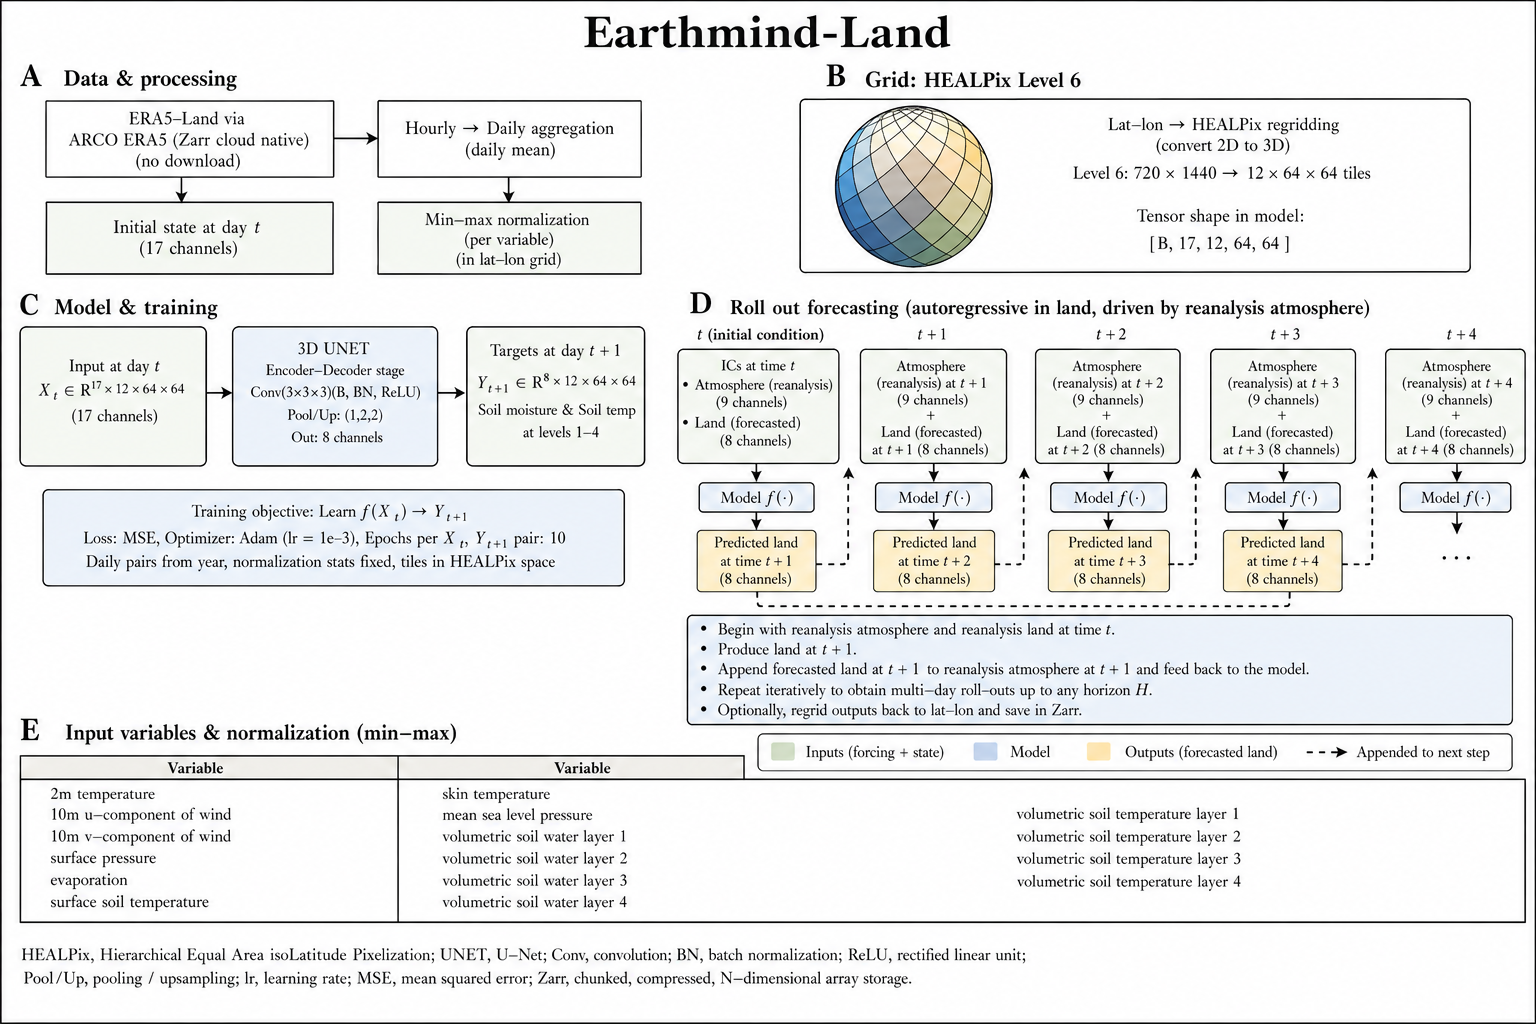
\includegraphics[width=\textwidth]{ai_land_model_schematic_v1.png}
    \caption{Architecture of the Earthmind-Land model. Initial conditions (IC) and atmospheric forcing fields in latitude--longitude format are regridded to HEALPix level~6 ($12 \times 64 \times 64$), passed through a 3D UNet encoder--decoder with skip connections, and the output is regridded back to latitude--longitude for evaluation. The 12 HEALPix faces serve as the depth dimension for 3D convolutions. Downsampling and upsampling operate only on the spatial dimensions within each face, preserving the face structure throughout.}
    \label{fig:architecture}
\end{figure}

\subsection{Training}
\label{sec:training}

\paragraph{Data preparation.} Training data are prepared for years 2018, 2019, and 2020. For each year, hourly ERA5 data are aggregated to daily means, yielding approximately 364 input--target pairs per year (day $t$ as input, day $t+1$ as target). Each sample is preprocessed according to Section~\ref{sec:preprocessing} and regridded from latitude--longitude to HEALPix in real time. To avoid redundant computation, the HEALPix tensor pairs are cached to disk after the first epoch and loaded directly for subsequent training.

\paragraph{Optimization.} The model is trained to minimize the mean squared error (MSE) loss between predicted and target soil variables in normalized space:
\begin{equation}
    \mathcal{L} = \frac{1}{N} \sum_{i=1}^{N} \| \hat{\mathbf{y}}_i - \mathbf{y}_i \|^2,
    \label{eq:mse}
\end{equation}
where $\hat{\mathbf{y}}_i$ and $\mathbf{y}_i$ are the predicted and target tensors for sample $i$, and $N$ is the batch size. We use the Adam optimizer with a learning rate of $10^{-3}$ and a batch size of 20. Training proceeds for 100 epochs, with the best model checkpoint selected based on the lowest evaluation loss. Training was performed on NVIDIA A100 GPUs at the Texas Advanced Computing Center (TACC).

\begin{table}[htbp]
\centering
\caption{Training configuration and deep learning model details for Earthmind-Land.}
\label{tab:training}
\small
\begin{tabular}{@{}ll@{}}
\toprule
\textbf{Parameter} & \textbf{Value} \\
\midrule
\multicolumn{2}{l}{\textit{Data and Training Setup}} \\
Training years & 2018--2020 (1092 samples) \\
Input normalization & MinMax to [0, 1] range (Eq.~\ref{eq:minmax}) \\
Output normalization & Same as input; denormalized during inference \\
Layer normalization & Batch normalization (after each conv layer) \\
Temporal resolution & Daily means (aggregated from ERA5 hourly) \\
Spatial resolution & HEALPix level 6 ($12 \times 64 \times 64 = 49,152$ pixels) \\
\midrule
\multicolumn{2}{l}{\textit{Model Architecture}} \\
Architecture & 3D UNet encoder--decoder \\
Depth dimension & 12 HEALPix base faces \\
Spatial dimensions & $64 \times 64$ per face \\
Total parameters & 4,525,224 \\
\midrule
\multicolumn{2}{l}{\textit{Optimization}} \\
Optimizer & Adam \\
Learning rate & $10^{-3}$ \\
Batch size & 20 \\
Loss function & Mean squared error (MSE) \\
Epochs & 100 \\
Model selection & Lowest validation loss \\
Hardware & NVIDIA A100 GPU \\
Training time & $\sim$8 hours per epoch \\
\bottomrule
\end{tabular}
\end{table}

\subsection{Autoregressive Rollout Inference}
\label{sec:inference}

At inference time, the model operates in an autoregressive fashion analogous to how offline physics-based LSMs are run (Algorithm~\ref{alg:rollout}). Given initial land surface conditions at time $t_0$ (the 8-variable soil state from ERA5), the workflow proceeds as follows:

\begin{enumerate}
    \item \textbf{Day 1}: The 9 atmospheric variables (forcing) at time $t$ are concatenated with the 8 soil state variables at time $t$ to form a 17-channel input. This input is normalized, regridded to HEALPix, processed through the 3D UNet, and the output (8 soil variables) is denormalized and regridded back to latitude--longitude to yield the prediction at time $t+1$.
    \item \textbf{Day 2 onward}: The predicted soil state from day 1 (not the ERA5 reanalysis) is used as the input soil state for day 2. However, the atmospheric forcing is taken from ERA5 reanalysis, not from the AI land model's output. This configuration is essential for offline evaluation: the atmosphere is held fixed at its observed evolution, eliminating the possibility that atmospheric model errors could mask land model performance. In a coupled system, both the land and atmosphere models would evolve their own states and exchange fluxes.
\end{enumerate}

This offline rollout approach directly mirrors how physics-based LSMs are validated: they are forced by observed atmospheric data while their internal state variables (soil moisture, temperature, snow) evolve freely. The prescribed atmospheric boundary conditions isolate land model skill from atmospheric model skill, providing a transparent baseline for assessing the land component's contribution to the coupled system.

\begin{algorithm}[htbp]
\caption{Autoregressive rollout forecast}
\label{alg:rollout}
\begin{algorithmic}[1]
\Require Initial conditions $\mathbf{s}_0$ (soil state at $t_0$), atmospheric forcing $\{\mathbf{a}_t\}_{t=0}^{T-1}$
\Ensure Forecast soil states $\{\hat{\mathbf{s}}_t\}_{t=1}^{T}$
\For{$t = 0$ to $T-1$}
    \State $\mathbf{x}_t \leftarrow \text{Concat}(\mathbf{a}_t,\; \mathbf{s}_t)$ \Comment{17-channel input}
    \State $\tilde{\mathbf{x}}_t \leftarrow \text{LatLon2HEALPix}(\text{Normalize}(\mathbf{x}_t))$
    \State $\tilde{\hat{\mathbf{s}}}_{t+1} \leftarrow f_\theta(\tilde{\mathbf{x}}_t)$ \Comment{3D UNet forward pass}
    \State $\hat{\mathbf{s}}_{t+1} \leftarrow \text{HEALPix2LatLon}(\text{Denormalize}(\tilde{\hat{\mathbf{s}}}_{t+1}))$
    \State $\mathbf{s}_{t+1} \leftarrow \hat{\mathbf{s}}_{t+1}$ \Comment{Predicted state becomes next input}
\EndFor
\end{algorithmic}
\end{algorithm}

When this model is eventually coupled with AI atmosphere and ocean models in the Earthmind S2S framework, the prescribed ERA5 atmospheric forcing will be replaced by forecasted atmospheric fields from the AI atmosphere model, and coupling will occur every 24 hours.

% =====================================================================
\section{Results}
\label{sec:results}

We evaluate the Earthmind-Land model in offline mode across two settings: short-range forecasts (1--9 days) to assess spatial fidelity, and extended-range forecasts (60 days) to assess S2S-scale skill across four high-impact extreme events.

\subsection{Short-Range Forecast Skill (1--9 Days)}
\label{sec:shortrange}

Short-range forecasts (days 1--9) assess the model's ability to reproduce large-scale spatial patterns and near-surface dynamics when errors from the initial conditions are still small. Initial conditions (ICs) are taken from ERA5 reanalysis at each evaluation date, providing a perfect initialization of the land surface state. For each case study event, we initialize forecasts at multiple dates (Table~\ref{tab:inits}), with ICs specified as the full 8-variable soil state (4 moisture layers + 4 temperature levels) from ERA5.

Figure~\ref{fig:rollout_sm} shows global maps of surface soil moisture (volumetric soil water layer~1) at forecast days 1, 5, and 9, comparing the model prediction against ERA5 ground truth. The model accurately reproduces the large-scale spatial patterns of soil moisture, including the contrast between arid regions (Sahara, Arabian Peninsula, Australian interior) and moist regions (tropics, mid-latitude continental interiors). As lead time increases, the spatial patterns remain well-captured, though some smoothing of fine-scale features becomes apparent.

\begin{figure}[htbp]
    \centering
    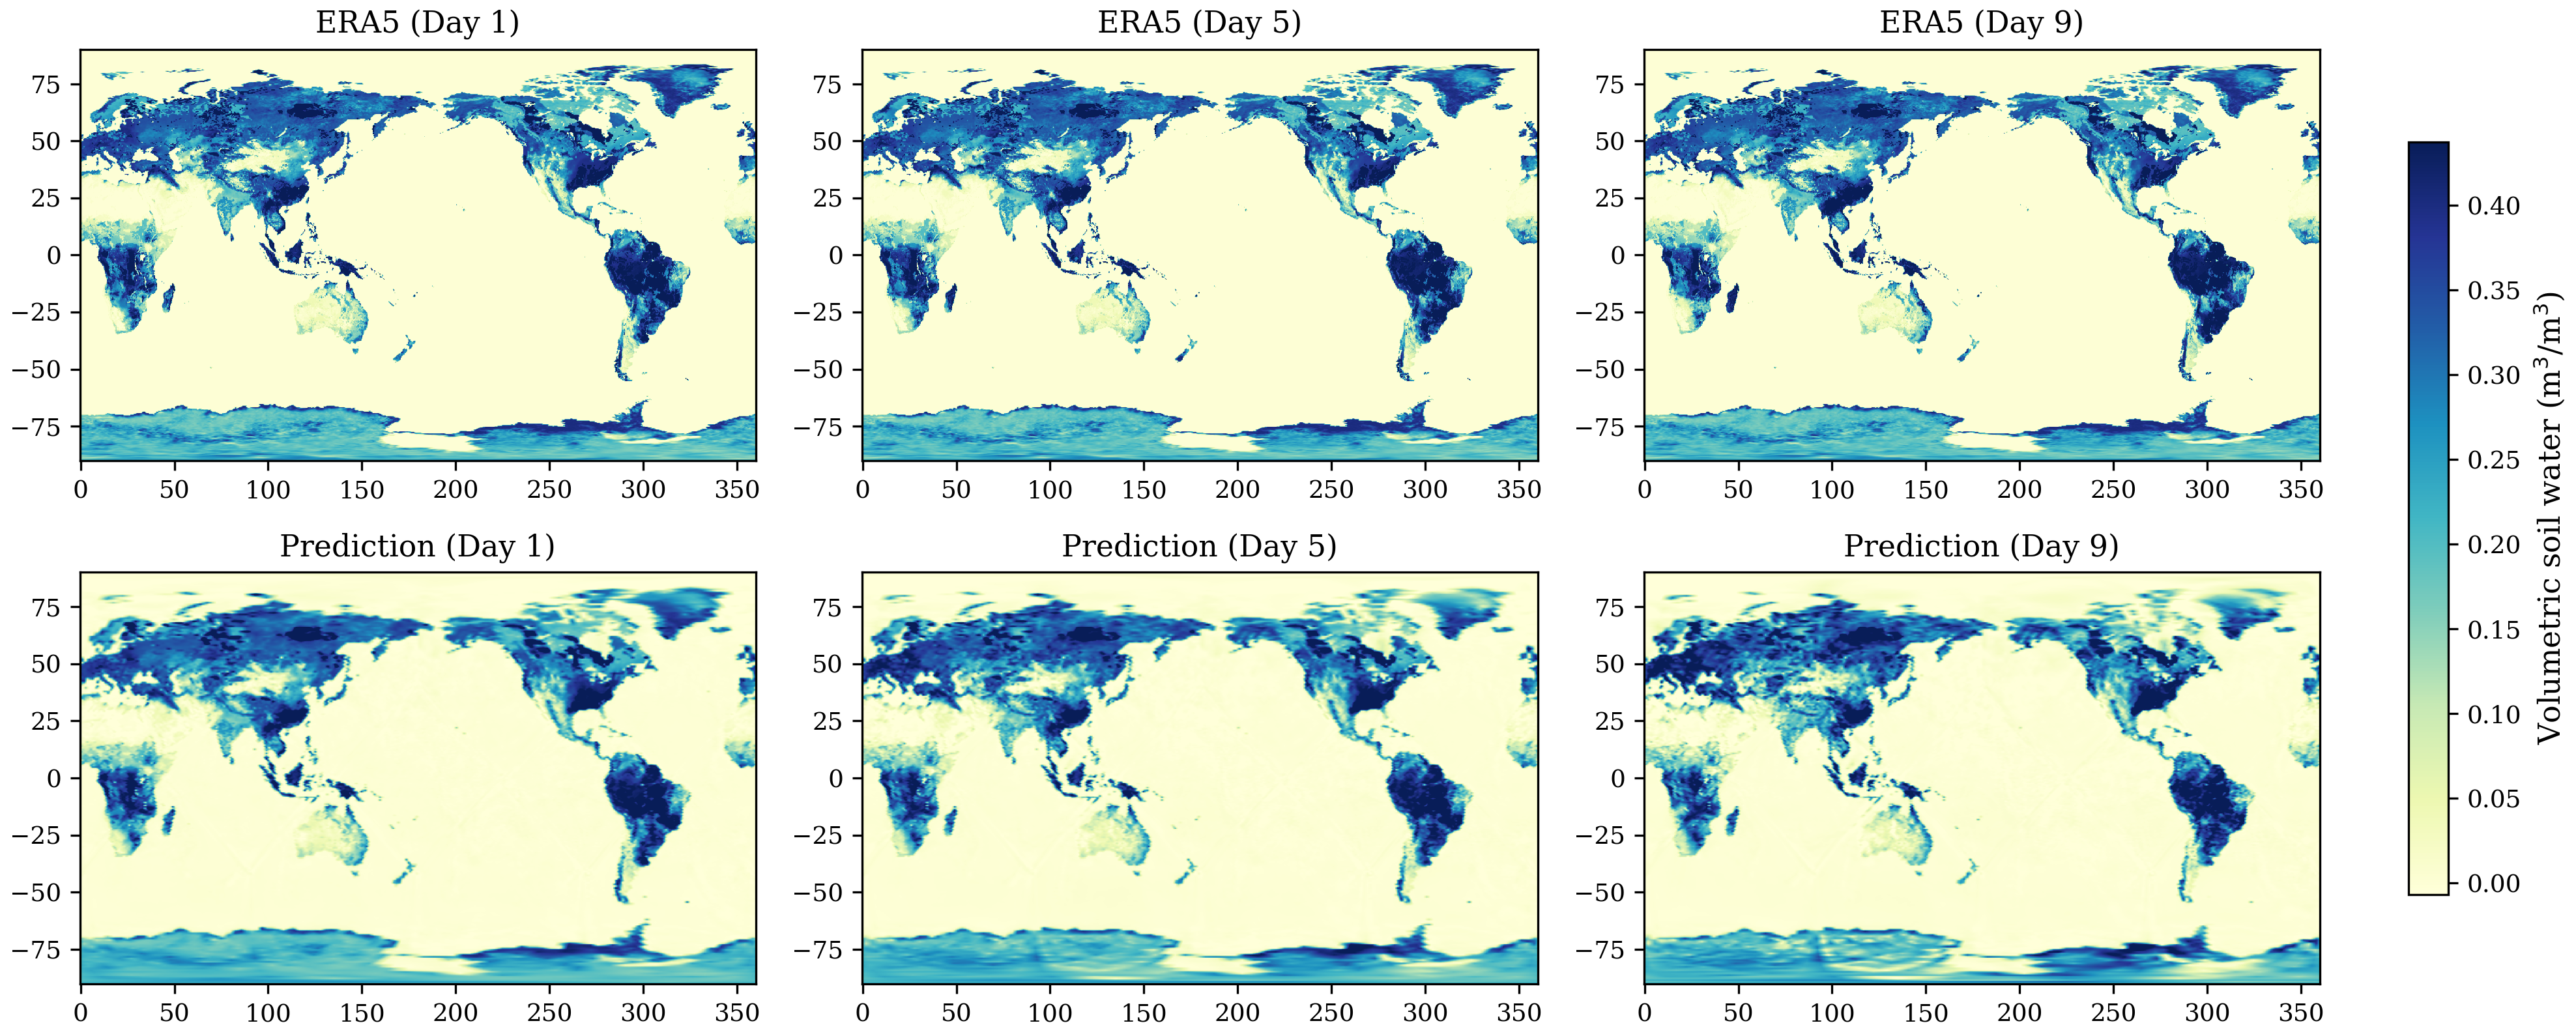
\includegraphics[width=\textwidth]{figures/fig_rollout_sm.png}
    \caption{Maps of volumetric soil water layer~1 (0--7\,cm) for the 2019 Mississippi River basin flooding case (IC: March 15, 2019), comparing ERA5 ground truth (top row) with model prediction (bottom row) at forecast days 1, 5, and 9. The model captures large-scale spatial patterns of soil moisture across all lead times.}
    \label{fig:rollout_sm}
\end{figure}

Figure~\ref{fig:rollout_st} presents the corresponding comparison for soil temperature level~1. The model reproduces the expected latitudinal temperature gradient and regional patterns, including warm tropical soils and cold polar regions, with high fidelity through day 9.

\begin{figure}[htbp]
    \centering
    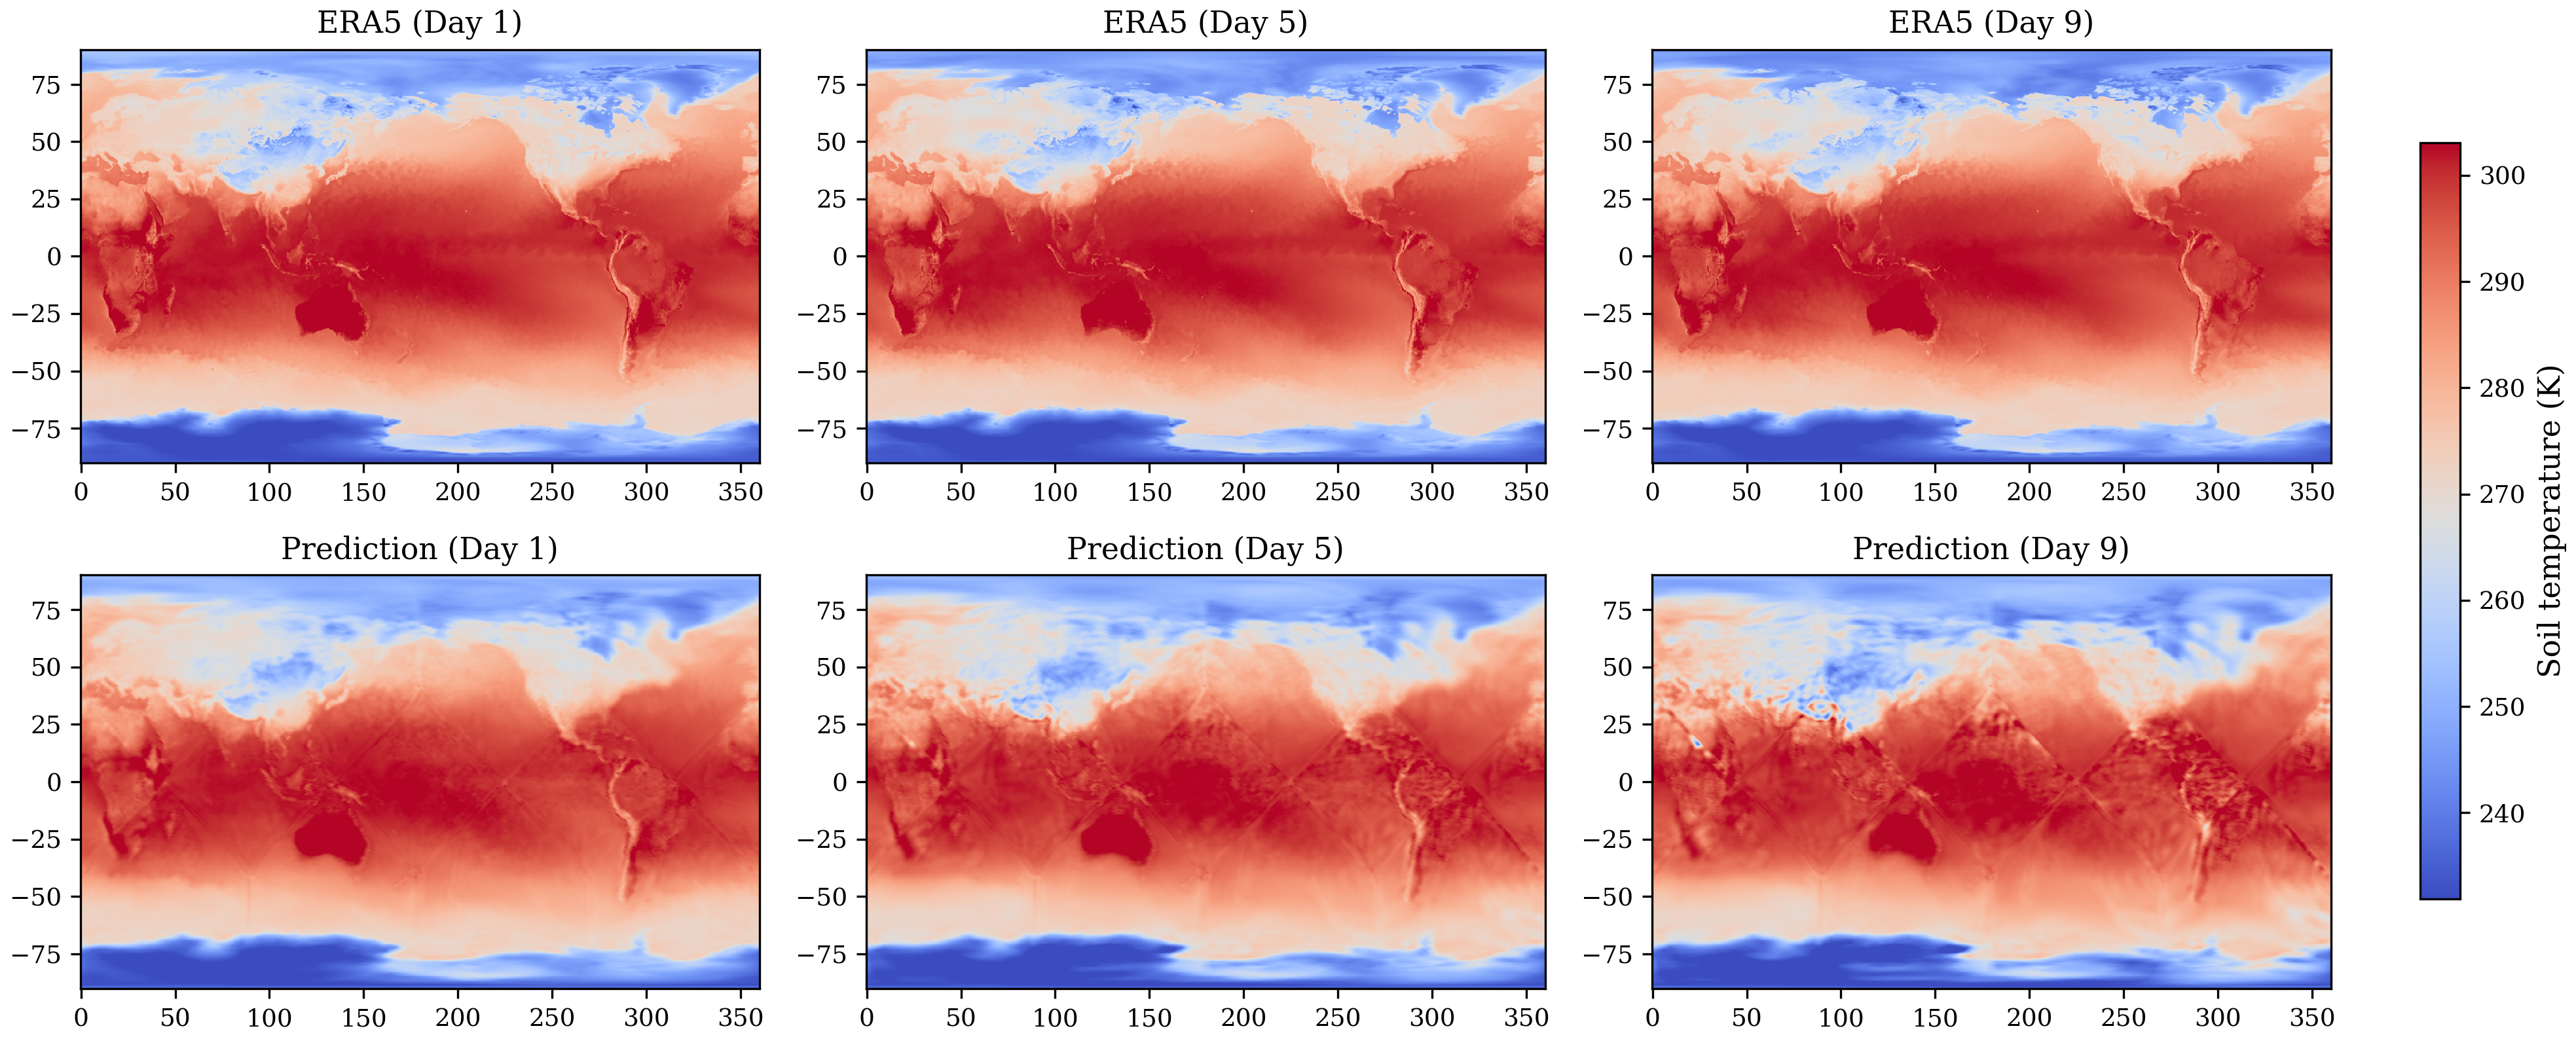
\includegraphics[width=\textwidth]{figures/fig_rollout_st.png}
    \caption{Soil temperature level~1 (0--7\,cm) for the 2019 Mississippi River basin flooding case (IC: March 15, 2019), comparing ERA5 ground truth (top row) with model prediction (bottom row) at days 1, 5, and 9. The model reproduces latitudinal gradients and regional patterns with high fidelity.}
    \label{fig:rollout_st}
\end{figure}

\subsection{Extended-Range Forecast Skill (60 Days)}
\label{sec:extendedrange}

To assess the model's skill at S2S scales, we perform 60-day autoregressive rollout forecasts for four high-impact extreme events across different regions:

\begin{enumerate}
    \item \textbf{2019 Mississippi River Basin Flooding} (initialized March 15, 2019; region 30--50$^\circ$\,N, 75--95$^\circ$\,W): Anomalous spring precipitation led to record flooding along the Mississippi River and its tributaries, with major agricultural impacts across the Midwest \citep{singh2023hybrid}.
    \item \textbf{2012 Central US Drought} (initialized May 15, 2012; region 35--45$^\circ$\,N, 90--105$^\circ$\,W): The most severe drought in the US since 1988, causing over \$30 billion in agricultural losses \citep{hoerling2014drought2012}.
    \item \textbf{2021 Pacific Northwest Heat Dome} (initialized June 10, 2021; region 45--50$^\circ$\,N, 115--125$^\circ$\,W): An unprecedented heat event that shattered temperature records across the Pacific Northwest of North America \citep{philip2022pnw}.
    \item \textbf{2011 Texas Drought} (initialized February 15, 2011; region 25--35$^\circ$\,N, 95--105$^\circ$\,W): A severe drought that caused an estimated \$7.6 billion in agricultural losses in Texas alone.
\end{enumerate}

For each event, additional initializations are tested (4 per event, 16 total) to assess robustness to initialization date. All evaluations exclude ocean grid points; only land pixels are assessed.

\subsubsection{Root Mean Square Error}

Figure~\ref{fig:rmse} shows the RMSE as a function of forecast lead time for soil moisture layers 1--4 across the four case studies and their initialization ensembles. Several features are noteworthy:

\begin{itemize}
    \item RMSE increases monotonically with lead time for all layers and events, consistent with expected error growth in autoregressive forecasts.
    \item Surface layers (layers 1 and 2) exhibit larger RMSE than deeper layers (layers 3 and 4), reflecting the higher variability and shorter memory timescales of near-surface soil moisture. Deep layers (layer 4) maintain low RMSE throughout the 60-day forecast window.
    \item The rate of error growth varies markedly across events: the 2012 Central US drought shows slower RMSE growth, likely because drought conditions evolve more slowly and with lower-frequency variability than rapidly evolving flooding events.
    \item Notably, the 2011 Texas drought (panel d) exhibits notably higher RMSE and steeper error growth compared to the other three cases, particularly for surface layers. This divergent behavior may reflect the complex interplay of precipitation deficit and high evaporative demand in the semi-arid Texas climate, combined with ERA5's known representational challenges in this region. The Texas domain ($25-35^\circ\text{N}, 95-105^\circ\text{W}$) is characterized by sparse observational networks, which may lead to larger ERA5 analysis uncertainties.
    \item Even at 60-day lead times, RMSE values remain physically reasonable, indicating the model maintains stability during extended autoregressive rollouts without unbounded error growth.
\end{itemize}

\begin{figure}[htbp]
    \centering
    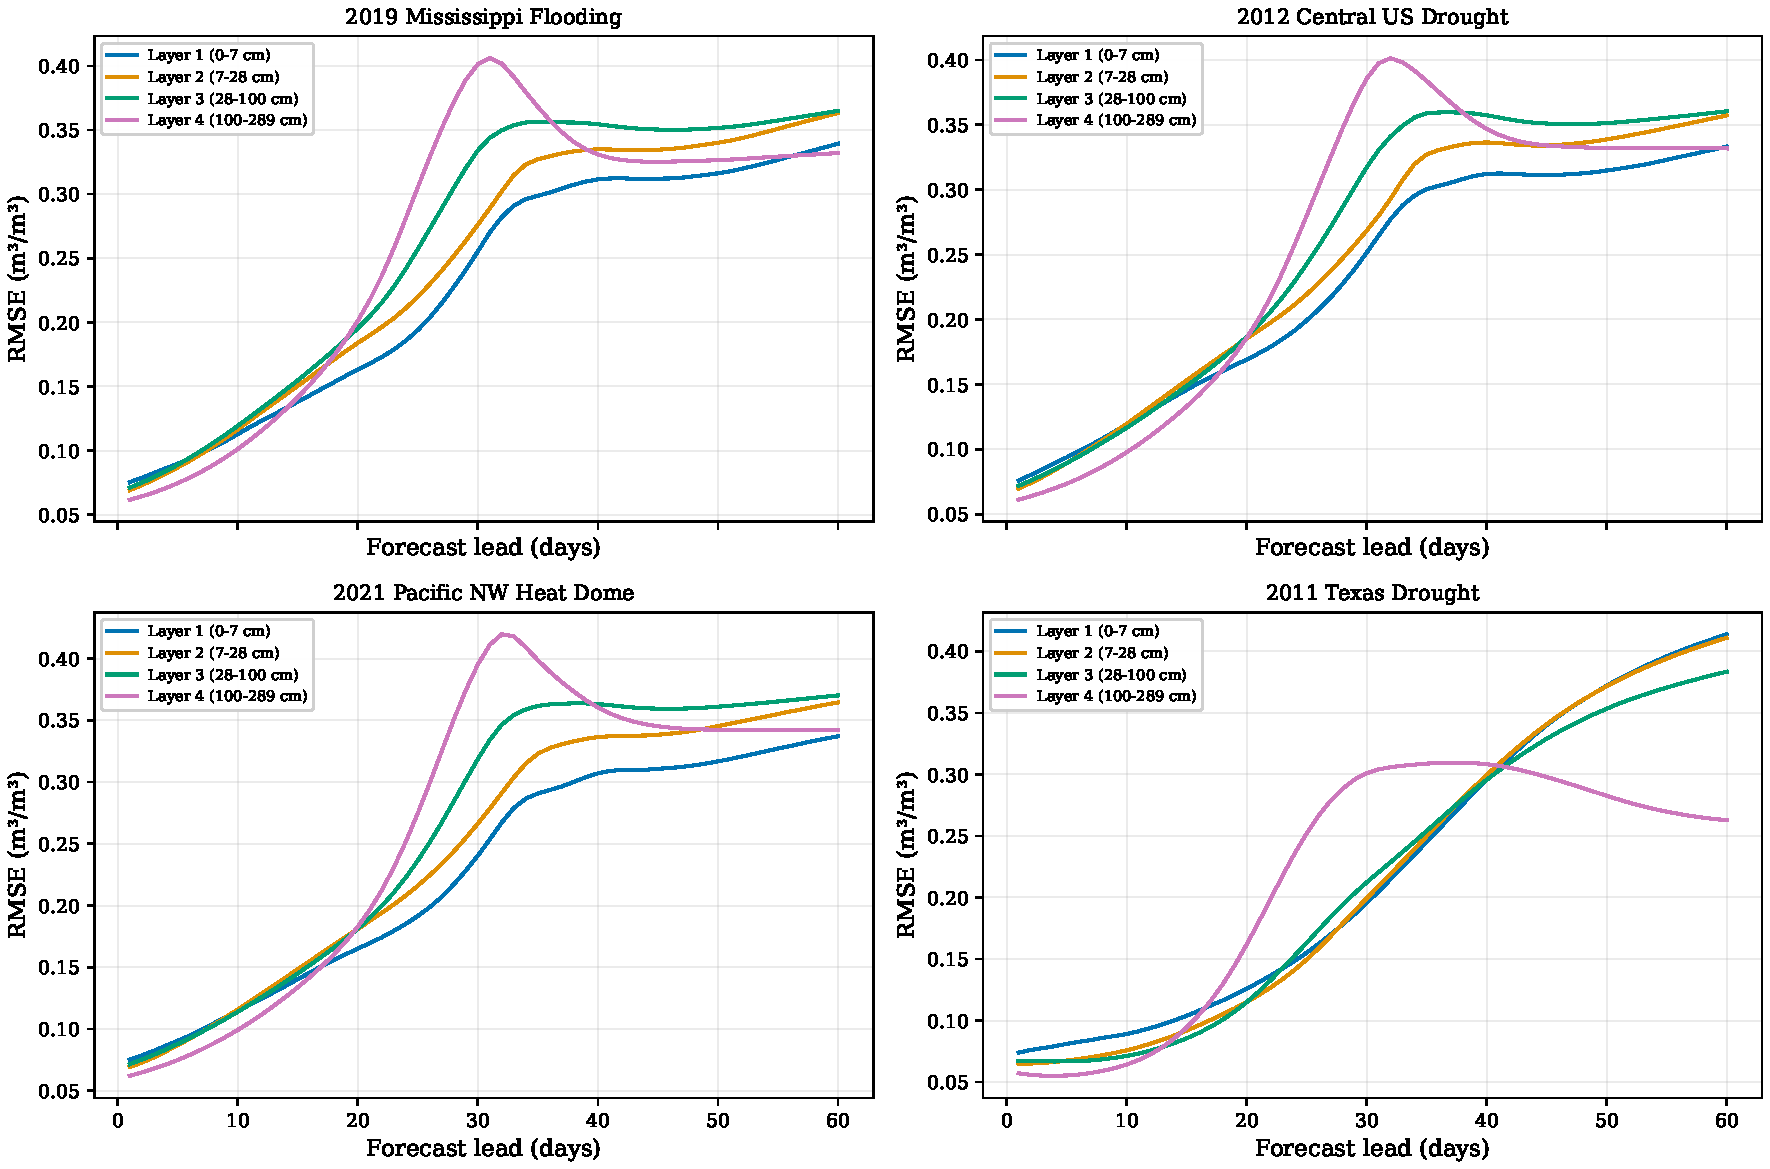
\includegraphics[width=\textwidth]{figures/fig_rmse.pdf}
    \caption{Root mean square error (RMSE) as a function of forecast lead time for volumetric soil water layers~1--4. Panels show (a) 2019 Mississippi River basin flooding, (b) 2012 Central US drought, (c) 2021 Pacific Northwest heat dome, and (d) 2011 Texas drought. Deeper layers show lower RMSE and slower error growth, consistent with longer soil moisture memory at depth. The Texas case (d) exhibits notably steeper error growth than the other regions, likely due to the semi-arid climate and sparse observational network in that domain.}
    \label{fig:rmse}
\end{figure}

\subsubsection{Anomaly Correlation Coefficient}

The anomaly correlation coefficient (ACC) provides a skill metric relative to climatology. We compute ACC as:
\begin{equation}
    \text{ACC} = \frac{\sum_{i} (f_i - \bar{f})(o_i - \bar{o})}{\sqrt{\sum_{i} (f_i - \bar{f})^2} \sqrt{\sum_{i} (o_i - \bar{o})^2}},
    \label{eq:acc}
\end{equation}
where $f_i$ and $o_i$ are the forecast and observed (ERA5) values at grid point $i$, and $\bar{f}$ and $\bar{o}$ are their respective spatial means.

Figure~\ref{fig:acc} shows ACC as a function of lead time for surface soil moisture (layer~1) across all four events. The model maintains ACC values above 0.8 through 15--20 days and above 0.5 through 30--40 days for most events. The 2012 drought case shows particularly high ACC retention, likely because the drought signal is large-scale and persistent, making it more predictable than rapidly evolving flooding events.

\begin{figure}[htbp]
    \centering
    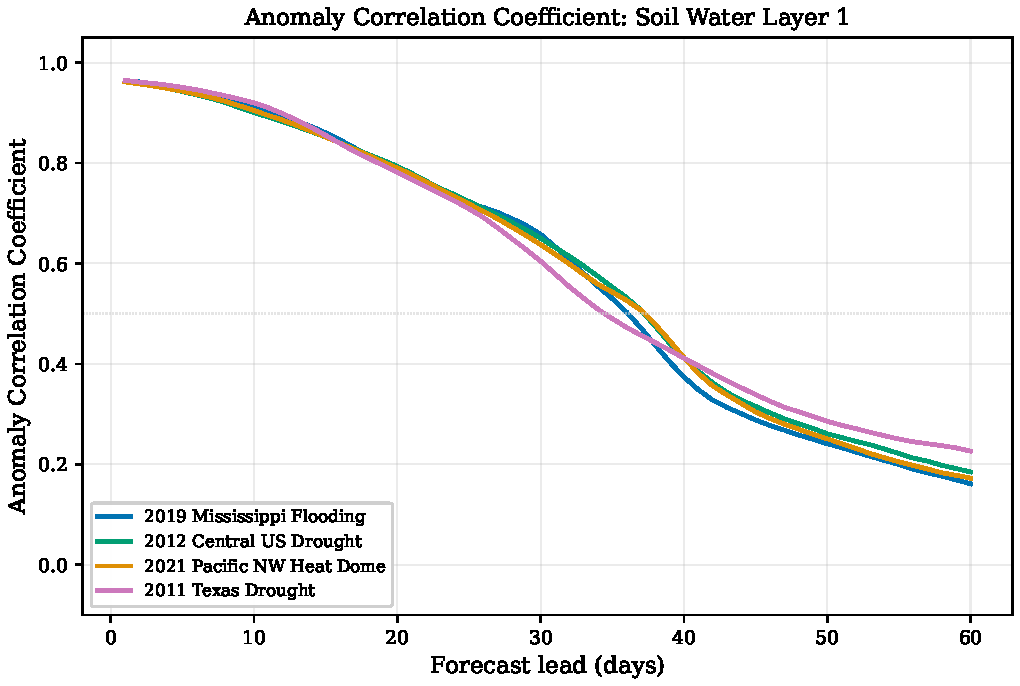
\includegraphics[width=\textwidth]{figures/fig_acc.pdf}
    \caption{Anomaly correlation coefficient (ACC) as a function of forecast lead time for volumetric soil water layer~1 across the four case studies: (a) 2019 Mississippi River basin flooding, (b) 2012 Central US drought, (c) 2021 Pacific Northwest heat dome, and (d) 2011 Texas drought. The dashed line indicates ACC = 0.5, a commonly used threshold for useful forecast skill. The model maintains useful skill (ACC $>$ 0.5) beyond 30 days for most events.}
    \label{fig:acc}
\end{figure}

\subsection{Multi-Initialization Robustness}
\label{sec:multi_init}

To assess the sensitivity of forecast skill to initialization date, we run 4 initializations per event (16 total; Table~\ref{tab:inits}). Figure~\ref{fig:multi_init} shows the RMSE spread across initializations for each event. The envelope of RMSE values is relatively narrow for most events and lead times, indicating that the model's skill is robust to initialization date within a given season and event type.

\begin{table}[htbp]
\centering
\caption{Initialization dates for the four case studies (16 forecasts total).}
\label{tab:inits}
\small
\begin{tabular}{@{}lllll@{}}
\toprule
\textbf{Event} & \textbf{Init 1} & \textbf{Init 2} & \textbf{Init 3} & \textbf{Init 4} \\
\midrule
2019 Mississippi Flooding & Mar 1 & Mar 15 & Apr 1 & May 1 \\
2012 Central US Drought & May 15 & Jun 1 & Jun 15 & Jul 1 \\
2021 Pacific NW Heat Dome & Jun 10 & Jun 17 & Jun 24 & Jun 27 \\
2011 Texas Drought & Feb 15 & Mar 1 & Apr 1 & Jun 1 \\
\bottomrule
\end{tabular}
\end{table}

\begin{figure}[htbp]
    \centering
    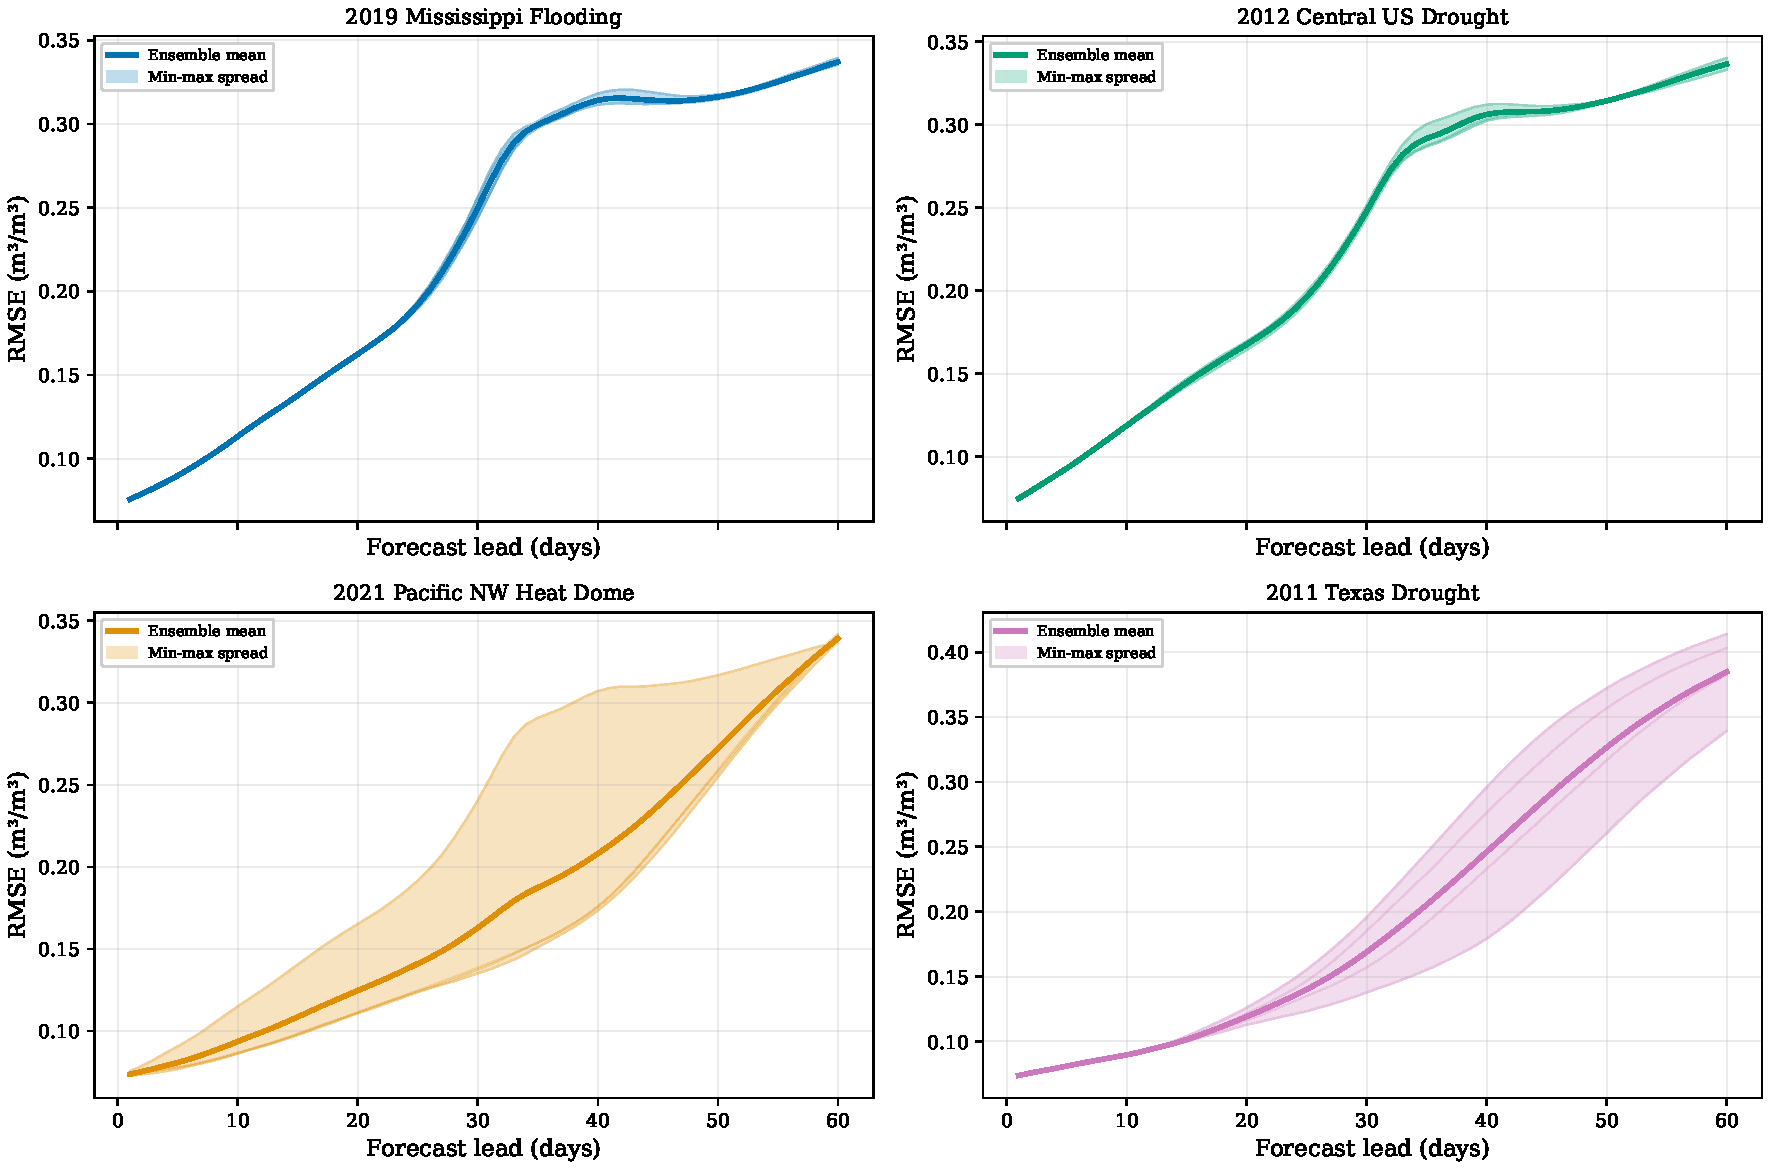
\includegraphics[width=\textwidth]{figures/fig_multi_init.pdf}
    \caption{RMSE versus lead time for volumetric soil water layer~1, showing all four initializations for each of the four case studies (16 forecasts total). Shaded regions indicate the envelope across initialization dates. The narrow spread within each event demonstrates robust forecast skill that is relatively insensitive to the precise initialization date within a season, validating the model's ability to capture predictable land surface signals.}
    \label{fig:multi_init}
\end{figure}

% =====================================================================
\section{Discussion}
\label{sec:discussion}

The Earthmind-Land model demonstrates that a relatively simple neural network architecture---a 3D UNet with 4.5 million parameters---can learn the temporal evolution of soil moisture and temperature at global scales when trained on ERA5 reanalysis data. Several aspects of this work merit further discussion.

\paragraph{Offline validation as a development paradigm.} The offline evaluation presented here requires explanation of what "offline" means in the context of land surface modeling. In an offline land surface model, the model receives prescribed atmospheric forcing (temperature, precipitation, radiation, wind, etc.) at each time step from observations or reanalysis, while the land surface state variables (soil moisture, soil temperature, etc.) evolve freely according to the model's dynamics. This contrasts with a coupled model, where the land surface and atmosphere exchange fluxes and feedbacks, allowing atmospheric predictions to respond to land surface anomalies. The Earthmind-Land model in offline mode receives ERA5 atmospheric fields as prescribed boundary conditions while its internal soil state evolves autoregressively.

This offline paradigm directly mirrors the development pathway of physics-based LSMs like Noah-MP \citep{niu2011noahmp} and CLM5. These models were extensively validated in offline mode against observed atmospheric data before being coupled into atmospheric GCMs. This approach isolates land model performance from atmospheric model errors, providing a clean assessment of the land model's intrinsic skill. Once a land model proves skillful in offline mode, it can then be coupled into a full earth system model where atmospheric and land surface feedback mechanisms are activated. The results presented here establish a baseline for future coupled evaluations within the Earthmind S2S framework.

\paragraph{Computational efficiency.} With 4.5 million parameters and approximately 17~MB of model weights, the Earthmind-Land model is orders of magnitude smaller than physics-based LSMs in terms of computational cost per forecast step. A 60-day rollout forecast takes seconds on a single GPU, compared to hours or more for physics-based models at comparable resolution. This efficiency is critical for ensemble S2S forecasting, where many forecast trajectories must be generated.

\paragraph{HEALPix as a unifying grid.} A key design choice is the use of HEALPix as the computational grid. This ensures direct compatibility with AI atmosphere and ocean models built on the same grid, eliminating the need for regridding at coupling boundaries. The HEALPix grid's equal-area property and demonstrated stability for long autoregressive rollouts \citep{karlbauer2024healpix} make it particularly well-suited for S2S-scale coupled modeling.

\paragraph{Error growth and soil moisture memory.} The ACC results reveal that forecast skill degrades faster for surface layers than for deeper layers, consistent with the shorter memory timescales of near-surface soil moisture. This is physically expected: surface soil moisture responds rapidly to precipitation and evaporation, while deep soil moisture evolves slowly and retains information for weeks to months. The model appears to have learned this depth-dependent memory structure from the data, without any explicit physical encoding.

\paragraph{Cloud-native training.} The use of ARCO-ERA5 Zarr data eliminates the need for large local data downloads, making the training pipeline accessible to researchers without extensive storage infrastructure. This approach also facilitates reproducibility, as the training data are publicly available and version-controlled.

% =====================================================================
\section{Limitations and Future Work}
\label{sec:limitations}

Several limitations of the current work should be acknowledged:

\begin{itemize}
    \item \textbf{Training data.} The model is trained exclusively on ERA5 reanalysis, which itself has biases in land surface variables, particularly in regions with sparse observations. ERA5 soil moisture is a model-derived product and may not accurately represent real-world soil moisture dynamics in all regions.

    \item \textbf{Process representation.} The model does not explicitly represent vegetation dynamics, snow processes, groundwater, or biogeochemical cycling. These processes are implicitly encoded in the ERA5 soil variables to the extent that they affect soil moisture and temperature, but the model cannot respond to novel forcings (e.g., land use change) not present in the training data.

    \item \textbf{Resolution.} The current HEALPix level~6 configuration yields an effective resolution of approximately 0.7$^\circ$, coarser than the native 0.25$^\circ$ ERA5 grid. Higher HEALPix levels (7 or 8) would capture finer-scale features but require proportionally more GPU memory and training time.

    \item \textbf{Training/test overlap.} The 2019 Mississippi flooding case study uses data from a year (2019) that is included in the training set. While the model is not trained on specific calendar dates but rather on day-to-day transitions, this overlap means the 2019 results should be interpreted with caution. The 2011, 2012, and 2021 cases are fully out-of-sample.

    \item \textbf{Deterministic forecasts.} The current model produces single deterministic forecasts without uncertainty quantification. Probabilistic forecasts through ensemble techniques or generative models (e.g., diffusion models) are essential for S2S applications.

    \item \textbf{Loss function.} The MSE loss function tends to produce smoothed predictions, particularly at longer lead times. Alternative losses (e.g., perceptual losses, adversarial training) or generative approaches may preserve sharper spatial features.
\end{itemize}

Future work will focus on:
\begin{enumerate}
    \item Coupling the AI land model with AI atmosphere and ocean models to form the complete Earthmind S2S system.
    \item Increasing resolution to HEALPix level 7 or 8.
    \item Incorporating additional state variables (snow depth, leaf area index, groundwater).
    \item Developing probabilistic forecasts using diffusion models or flow matching.
    \item Training on multiple reanalysis products and incorporating observational data from flux tower networks and satellite soil moisture retrievals.
    \item Exploring multi-step training losses to reduce error accumulation during autoregressive rollouts.
\end{enumerate}

% =====================================================================
\section{Conclusions}
\label{sec:conclusions}

We have presented Earthmind-Land, the first standalone AI land surface model designed for modular integration into coupled AI earth system models. The model employs a 3D UNet architecture with 4.5 million parameters operating on a HEALPix level~6 grid, trained on ERA5 reanalysis data accessed directly from a cloud-native Zarr store.

In offline mode, the model demonstrates skillful autoregressive forecasts of soil moisture and soil temperature out to 60 days across four high-impact extreme events spanning different hydroclimatic regimes: flooding, drought, and heat extremes. The model maintains anomaly correlation above 0.5 for surface soil moisture beyond 30 days and exhibits physically consistent depth-dependent error growth patterns.

The model's use of HEALPix as its computational grid, shared with companion AI atmosphere and ocean models, establishes the foundation for a fully coupled AI earth system model for S2S prediction. By following the physics-based model development paradigm of offline validation before coupled integration, this work provides a reliable baseline for assessing the added value of land--atmosphere--ocean coupling in AI-based S2S forecasting systems.

% =====================================================================
\section*{Data Availability}

ERA5 reanalysis data are publicly available through the ARCO-ERA5 Zarr store at Google Cloud Storage. The data can be accessed at:\\
\texttt{gs://gcp-public-data-arco-era5/ar/full\_37-1h-0p25deg-chunk-1.zarr-v3}\\
Model code and trained weights will be made available upon publication.

\section*{Acknowledgments}

Computational resources were provided by the Texas Advanced Computing Center (TACC) at The University of Texas at Austin. The HEALPix regridding was performed using the NVIDIA \texttt{earth2grid} library.

% =====================================================================
\bibliography{references}

\end{document}
